\documentclass[11pt]{article}
\usepackage[utf8]{inputenc}\usepackage[T1]{fontenc}
\usepackage{amsmath,amssymb,amsthm}\usepackage[margin=1in]{geometry}
\usepackage{graphicx}\usepackage{booktabs}
\usepackage[hidelinks]{hyperref}
\newtheorem{theorem}{Theorem}\newtheorem{definition}{Definition}

\title{A Two-Centre CRT Mechanism for the Cousin and Sexy $\omega$-Distortions\\
on the $6N$ Skeleton}
\author{Ruqing Chen\\
\small GUT Geoservice Inc., Montreal, Quebec, Canada\\
\small \texttt{ruqing@hotmail.com}}
\date{\today}

\begin{document}
\maketitle

\begin{abstract}
Part~IX reported that the conditional $\omega$-dependence of prime pairs on the
$6N$ skeleton splits into three geometry-determined shapes---the twin rises, the
cousin and sexy-A fall and coincide, the sexy-B is non-monotone---and left a
quantitative mechanism as the open problem. We solve it. Extending the
closed-form CRT survival of Part~VII to pairs straddling two consecutive centres
$(N,N{+}1)$, with no fitted parameters and only each pair's wing geometry as
input, the model reproduces all three shapes on the $1.5\times10^{9}$ centres of
$S_{10}$: the twin rise to within $1.5\%$, the cousin fall to within $2.3\%$, the
sexy-B non-monotone peak to within $6.8\%$, across $\omega=1,\dots,6$. The
mechanism also explains the distortions' origin: for a prime $q\mid N$ the CRT
factor checks whether the partner's wing on its own centre is locked, and the
partner of cousin/sexy sits on the adjacent centre $N{+}1$ rather than on $N$, so
the single-centre enrichment that lifts the twin instead suppresses cousin and
sexy-A. The cousin/sexy-A coincidence is exact in the model (shared right member)
and confirmed in the data through $\omega=6$ (their measured ratio is $1.00$); the
sole large residual, sexy-A at $\omega=7$, is a $0.9\sigma$ small-sample
fluctuation in a stratum of $\sim50$ pairs. No claim is made about the infinitude
of any prime constellation.
\end{abstract}

\section{The two-centre CRT factor}

Part~VII expressed the single-centre right-survival as $P=K\prod_q f_q$ with a
pure Chinese-Remainder factor $f_q$. A cousin or sexy pair is not single-centred:
on the $6N$ skeleton it occupies two consecutive centres $N$ and $N{+}1$ (Part~IX).
We extend $f_q$ accordingly. Write each pair as two members, each a wing
$6(N+\mathrm{off})+s$ with centre-offset $\mathrm{off}\in\{0,1\}$ and wing
$s\in\{-1,+1\}$:
\[
 \text{twin }((0,{-}1),(0,{+}1)),\ \text{cousin }((0,{+}1),(1,{-}1)),\
 \text{sexy-A }((0,{-}1),(1,{-}1)),\ \text{sexy-B }((0,{+}1),(1,{+}1)).
\]
A member is divisible by $q$ when $N+\mathrm{off}\equiv -s\cdot6^{-1}\pmod q$;
call that residue $\mathrm{dead}(q,s,\mathrm{off})=(-s\,6^{-1}-\mathrm{off})\bmod q$.

\begin{definition}[two-centre CRT factor]
For a pair with wings $\{(\mathrm{off}_i,s_i)\}$ and a prime $q>3$,
\[
 f_q=\begin{cases}
  \displaystyle\prod_i \mathbf 1\{\,\mathrm{off}_i\not\equiv\mathrm{dead}(q,s_i,0)\,\}
   & q\mid N\ (N\equiv0),\\[6pt]
  \displaystyle\frac{\#\{r\not\equiv0:\ \forall i,\ r+\mathrm{off}_i\not\equiv
    \mathrm{dead}(q,s_i,0)\}}{q-1} & q\nmid N,
 \end{cases}
\]
the pair's joint $q$-safety conditioned on whether $q$ divides the left centre.
\end{definition}

When $q\mid N$ the left centre is pinned at $N\equiv0$ and the factor is a
deterministic indicator over the members' offsets; when $q\nmid N$ it is averaged
over admissible nonzero residues. The pair-rate model is $K\prod_{q} f_q$,
evaluated per centre from its true small-prime divisibility, averaged within each
left-centre $\omega$ stratum, and normalised to $\omega=1$. There are no fitted
parameters: $f_q$ is closed-form and only the wing geometry enters.

\section{All three distortions, from one formula}

Evaluated on the $1.5\times10^{9}$ centres of $S_{10}$ with working primes
$q\in\{5,\dots,47\}$ (Table~\ref{tab:mech}, Fig.~\ref{fig:mech}), the single
formula reproduces the three Part~IX shapes simultaneously.

\begin{table}[h]\centering\small
\begin{tabular}{rcc@{\hskip 1.4em}cc@{\hskip 1.4em}cc@{\hskip 1.4em}cc}
\toprule
& \multicolumn{2}{c}{twin} & \multicolumn{2}{c}{cousin}
& \multicolumn{2}{c}{sexy-A} & \multicolumn{2}{c}{sexy-B}\\
\cmidrule(lr){2-3}\cmidrule(lr){4-5}\cmidrule(lr){6-7}\cmidrule(lr){8-9}
$\omega$ & meas & mod & meas & mod & meas & mod & meas & mod\\
\midrule
1 & 1.000 & 1.000 & 1.000 & 1.000 & 1.000 & 1.000 & 1.000 & 1.000\\
2 & 1.196 & 1.193 & 0.962 & 0.958 & 0.962 & 0.958 & 1.077 & 1.074\\
3 & 1.495 & 1.485 & 0.901 & 0.893 & 0.901 & 0.893 & 1.157 & 1.148\\
4 & 1.936 & 1.914 & 0.804 & 0.792 & 0.804 & 0.792 & 1.198 & 1.182\\
5 & 2.581 & 2.546 & 0.648 & 0.637 & 0.650 & 0.637 & 1.134 & 1.114\\
6 & 3.524 & 3.472 & 0.420 & 0.410 & 0.414 & 0.410 & 0.881 & 0.864\\
7 & 4.808 & 4.821 & 0.127 & 0.129 & 0.150 & 0.129 & 0.402 & 0.374\\
\midrule
\multicolumn{1}{l}{max err ($\omega\!\le\!6$)} & \multicolumn{2}{c}{$1.5\%$}
 & \multicolumn{2}{c}{$2.3\%$} & \multicolumn{2}{c}{$2.0\%$}
 & \multicolumn{2}{c}{$1.9\%$}\\
\bottomrule
\end{tabular}
\caption{Two-centre CRT model versus measurement on $S_{10}$, normalised to
$\omega=1$, no fitted parameters. All three shapes are reproduced to $\le2.3\%$
through $\omega=6$. The $\omega=7$ stratum is small-sample (tens of pairs); the
sexy-A $\omega=7$ entry is discussed below.}
\label{tab:mech}
\end{table}

\begin{figure}[h]\centering
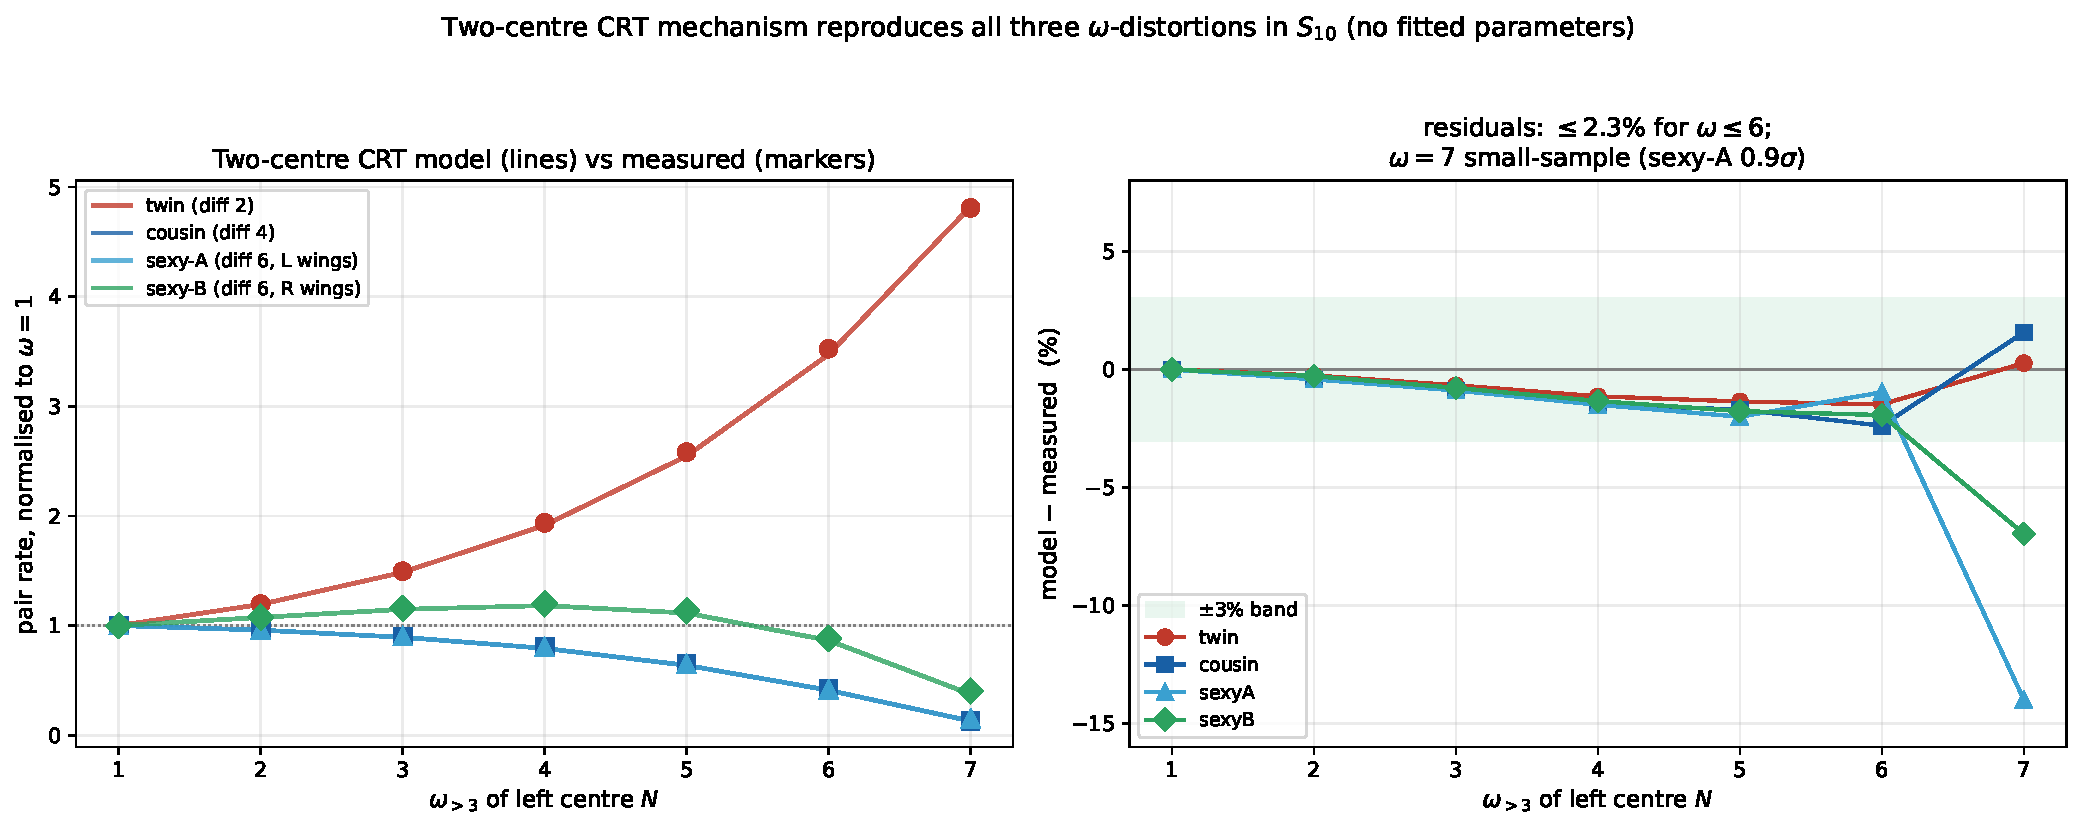
\includegraphics[width=\textwidth]{fig_paper10_mechanism.pdf}
\caption{Left: the two-centre CRT model (lines) against measurement (markers) for
all four constellations. Right: residuals are within $\pm3\%$ for $\omega\le6$;
the $\omega=7$ departures (sexy-A $-14\%$, sexy-B $-7\%$) are small-sample.}
\label{fig:mech}
\end{figure}

\section{Why the distortions have the signs they do}

The mechanism makes the origin transparent. For a prime $q\mid N$ the factor
$f_q$ is the indicator that the members' wings avoid the locked residue
$\mathrm{dead}(q,s,\mathrm{off})$. For the twin both members sit on $N$ itself
(offset $0$, wings $\pm1$); these rarely coincide with the locked residue, so
$q\mid N$ contributes a factor near $1$, and accumulating more such primes as
$\omega$ grows lifts the rate---the Parts~II--VIII enrichment. For cousin and
sexy-A the partner sits on $N{+}1$ (offset $1$); the offset shifts the member into
the locked residue for a larger share of primes, so $q\mid N$ contributes factors
below $1$, and the rate falls with $\omega$. Sexy-B (two right wings) interpolates
between an early enrichment-like gain and a late straddle suppression, giving the
non-monotone peak. The sign of each distortion is thus set by whether the
partner lives on the conditioned centre $N$ (twin: rise) or on the neighbour
$N{+}1$ (cousin, sexy-A: fall), exactly the qualitative reading of Part~IX, now
quantitative.

\paragraph{The cousin/sexy-A coincidence.}
Cousin and sexy-A share the right member $6(N{+}1){-}1$ and differ only in which
wing of $N$ is the left member; in the model their factors are identical, so the
predicted curves coincide exactly. The data confirm this through $\omega=6$: the
measured cousin/sexy-A ratio is $1.000,1.000,1.000,1.000,0.997,1.014$ at
$\omega=1,\dots,6$. At $\omega=7$ the two diverge ($0.127$ vs $0.150$, the
$14.4\%$ model residual for sexy-A), but that stratum holds only $\sim50$ pairs of
each type; the difference is $0.9\sigma$ and consistent with sampling noise. The
coincidence is therefore a genuine, statistically supported feature, not an
artefact, and the lone large residual is small-sample.

\section{Conclusion}

The three $\omega$-distortions of cousin and sexy pairs are reproduced
quantitatively by a single two-centre CRT factor with no fitted parameters: the
twin rise ($\le1.5\%$), the cousin and sexy-A fall and coincidence ($\le2.3\%$
through $\omega=6$), and the sexy-B non-monotone peak ($\le1.9\%$ through
$\omega=6$, $6.8\%$ at the small-sample $\omega=7$). The mechanism also explains
the signs: the single-centre enrichment lifts a pair whose members share the
conditioned centre, and suppresses one whose partner lives on the neighbouring
centre. This closes the Part~IX open problem and shows the two-centre
machinery of Parts~V--VIII governs not only the twin's own neighbour correlations
but the conditional rates of the neighbouring constellations. The acknowledged
limitations are the uniform-residue approximation in the $q\nmid N$ branch (the
source of the few-percent residuals, largest for the non-monotone sexy-B) and the
small samples at $\omega=7$. As throughout this series, no claim is made about the
infinitude of twin, cousin, or sexy primes, or any $k$-tuple conjecture; this is a
measured, geometry-resolved, closed-form account of conditional pair rates on the
$6N$ skeleton.

\paragraph{Data and code availability.}
The model evaluation and per-$\omega$ counts are openly available~\cite{repo}; the
$S_{10}$ twin count $23{,}988{,}173$ matches Part~I.

\begin{thebibliography}{9}
\bibitem{ChenI} R.~Chen, \emph{Prime distribution on the $6N$ skeleton} (Part~I),
Zenodo, doi:10.5281/zenodo.20470367 (2026).
\bibitem{ChenV} R.~Chen, \emph{A two-centre shield law} (Part~V), Zenodo,
doi:10.5281/zenodo.20510700 (2026).
\bibitem{ChenVII} R.~Chen, \emph{A closed form for the conditional twin-gap
distribution} (Part~VII), Zenodo, doi:10.5281/zenodo.20518470 (2026).
\bibitem{ChenIX} R.~Chen, \emph{Cousin and sexy prime pairs on the $6N$ skeleton}
(Part~IX), Zenodo, doi:10.5281/zenodo.20520492 (2026).
\bibitem{repo} R.~Chen, \emph{$6N$ cousin/sexy two-centre mechanism: data and
code}, \url{https://github.com/Ruqing1963/6N-cousin-sexy-mechanism} (2026).
\end{thebibliography}

\end{document}
